\chapter{Work Plan}%
\label{chapter:workPlan}

\begin{introduction}
This chapter explains the work plan for the development of the applications and the dissertation writing.
\end{introduction} 


\section{Work Plan}

In the following months, the first version of the applications is planned to be accomplished according to the use cases defined in Chapter III. 
The development, as illustrated in figure \ref{fig:figure1}, will be structured in 6 two-week long sprints, with 2 contingency weeks. One between sprint 3 and 4 and another after sprint 6, in case of delays on some tasks.

The Sprint 1 will be dedicated to the integration with the LightMobie System and the development of the Receptionist Use Cases, as seen below: 

\begin{itemize}
  \item Integration with the System;
  \begin{itemize}
      \item Start Date: 24/01/2025 
      \item End Date: 27/01/2025 
  \end{itemize}
    \item Receptionist Use Cases;
    \begin{itemize}
        \item Start Date: 28/01/2025 
        \item End Date: 06/02/2025 
    \end{itemize}
  \end{itemize}

In Sprint 2, the development of the first five Use Cases of the mechanic is planned as follows:  

\begin{itemize}
  \item Mechanic Use cases 2.1 - 2.5;
    \begin{itemize}
      \item Start Date: 07/02/2025 
      \item End Date: 20/02/2025 
  \end{itemize}
\end{itemize}

The Sprint 3 will be dedicated to the last two Use Cases of the mechanic:  

  \begin{itemize}
    \item Mechanic Use Cases 2.6 and 2.7;
    \begin{itemize}
      \item Start Date: 21/02/2025 
      \item End Date: 06/03/2025 
  \end{itemize}
\end{itemize}

The following week is reserved for the contingency, so in the case of no delay, Sprint 4 is succeeding.
In the Sprint 4, the Admin Use Cases from 4.3 to 4.5 are planned. The 4.1 and 4.2 were skipped to further weeks since they are related to the Warehouse Use Cases.

    \begin{itemize}
      \item Admin Use Cases 4.3 - 4.5;
    \begin{itemize}
      \item Start Date: 14/03/2025 
      \item End Date: 27/03/2025 
  \end{itemize}
\end{itemize}

The Sprint 5 is expected to the development of the remaining two Admin Use Cases and the Warehouse Use Cases.

\begin{itemize}
  \item Admin Use Cases 4.1 and 4.2;
  \begin{itemize}
    \item Start Date: 28/03/2025 
    \item End Date: 06/04/2025 
  \end{itemize}
  \item Warehouse Use Cases;
  \begin{itemize}
    \item Start Date: 07/04/2025 
    \item End Date: 10/04/2025 
  \end{itemize}
\end{itemize}

The final sprint, Sprint 6, will be reserved for developing the client application Use Cases.

\begin{itemize}
  \item Client App Use Case;
  \begin{itemize}
    \item Start Date: 11/04/2025  
    \item End Date: 24/05/2025 
  \end{itemize} 
\end{itemize}
The following week is reserved for another contingency.

 Following the development of the applications, another two weeks are foreseen to conduct a user testing, to apply the notes and suggestions of the experiment, and to code improvements.
 The remaining time will be used to finish writing the dissertation, primarily the results and conclusion.
  
 The literature will accompany this process, since it may appear another paper or study that may be relevant to the work.


    \begin{figure}[h]
      \caption{Planned Work described as a Gantt Chart. The dissertation is estimated to be at 25\%, the literature progress to be 70\%, the application Use cases at 85\%, and the admin Use Cases at 10\%. The admin Use Cases are at 10\% since they are partly developed in the LightMobie System.}
      \centering
      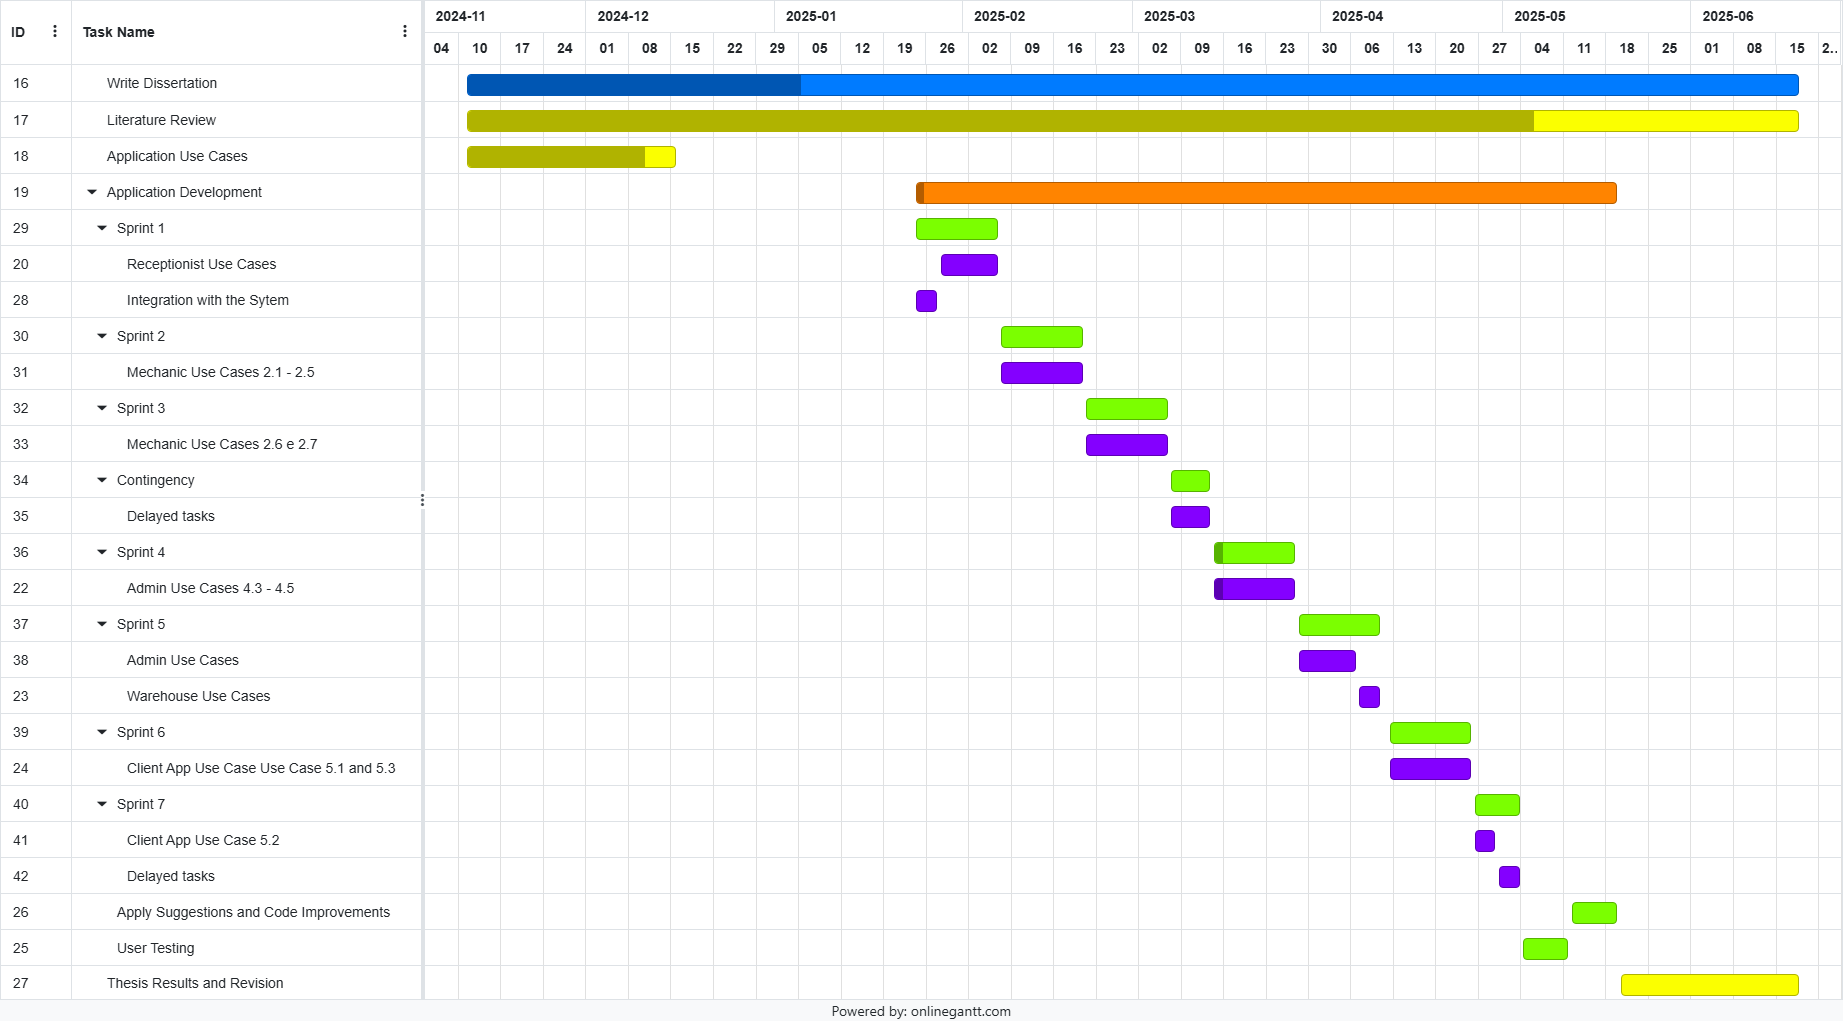
\includegraphics[width=\textwidth]{figs/Gantt}
      \label{fig:figure1}
    \end{figure}
